\chapter{\label{chapter5}Evaluation}

In this chapter, we present the results of the tests we ran to evaluate the convergence performance of the iSDX. We explain the test setup in \ref{chapter5:Test Setup}. We present the convergence time of the iSDX without Swift in \ref{chapter5:Convergence time without Swift}, the convergence time of the iSDX with Swift in \ref{chapter5:Convergence time with Swift} and examine the Swift overhead in \ref{chapter5:Swift overhead}.

The results show that iSDX with Swift converges about 60 times faster. However, this comes at the cost of a $13\%$ increase in processing time for BGP updates. The majority of the convergence time is spent on detecting the burst.

In the next chapter we discuss the results, examine the VMAC partitioning and the fast reroute rules.

\section{\label{chapter5:Test Setup}Test Setup}

\begin{figure}[h]
\center
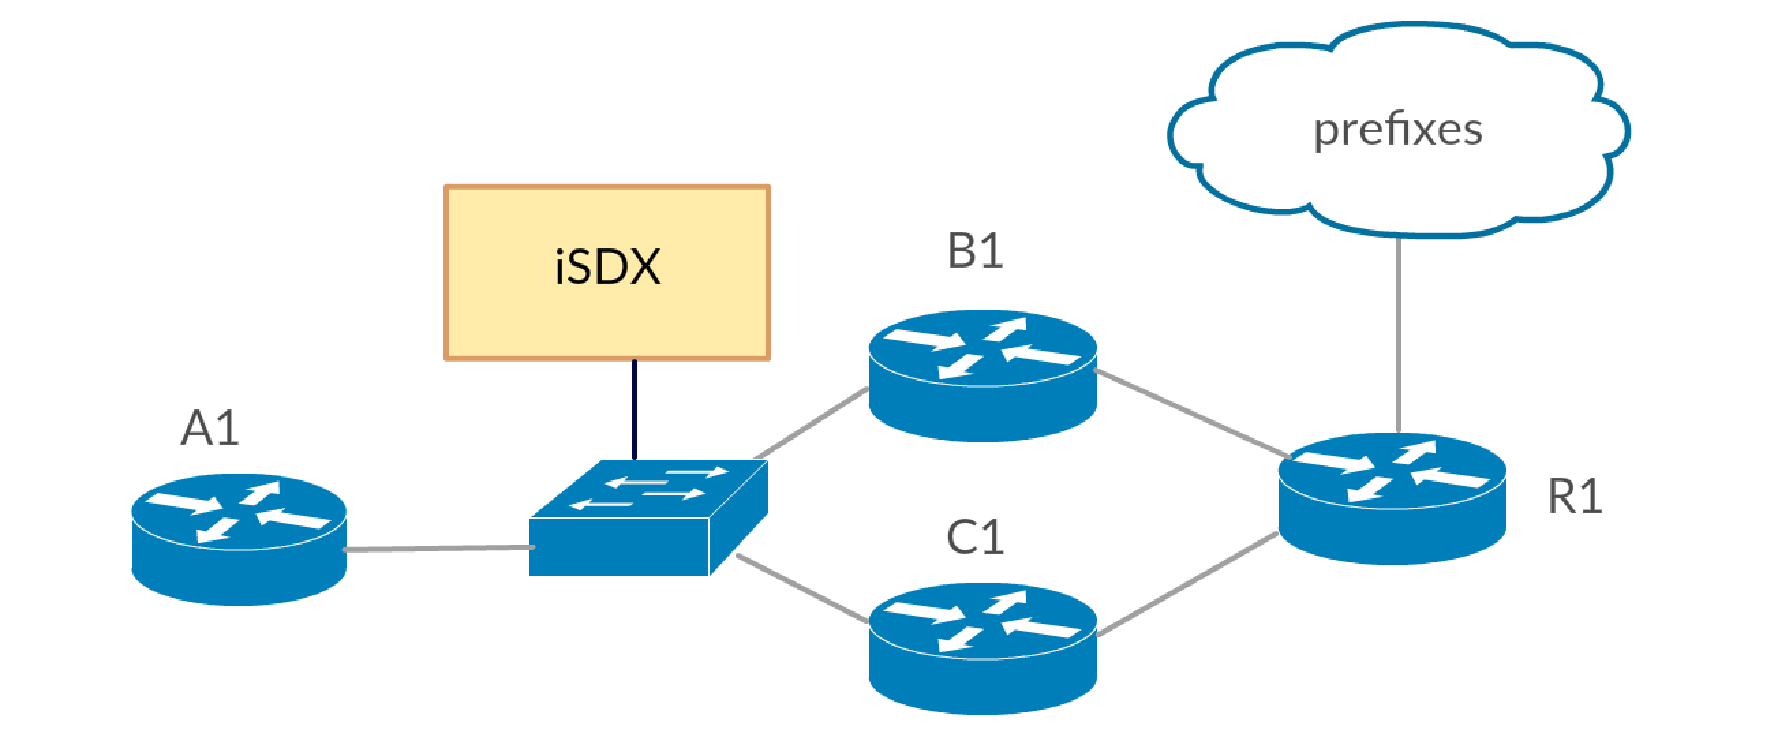
\includegraphics[scale = 0.36]{Figures/eval_exp_setup.pdf}
\caption{Test Setup}
\label{fig:test-setup}
\end{figure}

Figure~\ref{fig:test-setup} shows the test setup.
The test setup has an iSDX with or without Swift connected to three participants. Participants B1 and C1 are connected to the rest of the internet via R1 and advertise up to 500000 prefixes to A1. Participant A1 prefers routes from B1. Remote failure is simulated by setting the link between B1 and R1 down. If this link is down A1 needs to updates his RIB, check if flow rules have changed and update the virtual next-hop/VMAC for every withdrawn prefix.

The experiment setup is run on a server running Ubuntu 14.04 with the following specs: Intel Xeon CPU E5620 with 4 Cores at 2.4 GHz, 36GB of RAM. We use Mininet~\cite{mininet} to simulate the network. The routers A1, B1, C1 and R1 are quagga~\cite{quagga} routers. The perl script bgpsimple~\cite{bgpsimple} is used to inject an arbitrary number of routes into R1. 

\section{\label{chapter5:Convergence time without Swift}Convergence Time without Swift}

We measure the convergence time as the time between the first withdraw arriving at the route server and the participant controller finishing to process the last withdraw. To measure the convergence time we use the built in iSDX log server.

This convergence time does not take into account the hold timer or the time the participant router takes to process the withdrawals. But since these things are not under the control of the iSDX they are ignored in this evaluation.

\begin{figure}
\centering
\begin{minipage}[t]{.4\textwidth}
\centering
\vspace{0pt}
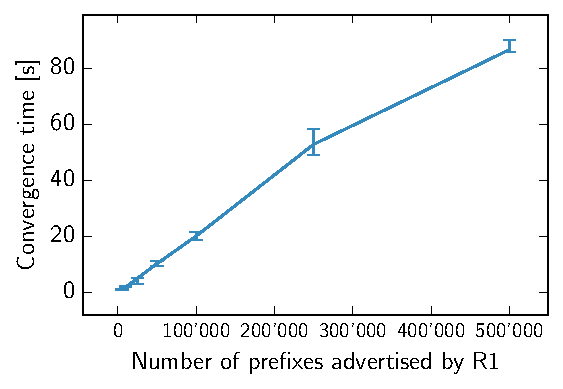
\includegraphics[scale = 1]{Figures/noswift.pdf}
\end{minipage}\hfill
\begin{minipage}[t]{.4\textwidth}
\centering
\vspace{0pt}
\begin{tabular}{@{}lr@{}}
	\\
	prefixes & Conv. time \\
	\hline
	\\
    5K & 0.9 s  \\
    10K & 1.8 s   \\
    25K & 4.9 s   \\
    50K & 10.1 s  \\
    100K & 20 s \\
    250K & 52.75 s   \\
    500K & 86.5 s  \\
\end{tabular}
\end{minipage}
\caption{Convergence time of the iSDX without Swift}
\label{fig:noswift}
\end{figure}

Figure~\ref{fig:noswift} shows the convergence time in relation to the number of prefixes injected by bgpsimple. The results show that the convergence time increases linearly with the number of prefixes advertised by R1.

At $500'000$ prefixes the iSDX takes about $90$\,seconds to converge. During these $90$\,seconds A1 is still sending packet to B1 even though that route does not exist anymore. Hence, all the traffic is dropped. 

\section{\label{chapter5:Convergence time with Swift}Convergence Time with Swift}

In this section, we measure the convergence time as the time between the first withdraw arriving at the route server and the participant controller's FR-handler finishing to push the Fast-reroute rules.

\begin{figure}[h]
\centering
\begin{minipage}[t]{.4\textwidth}
\centering
\vspace{0pt}
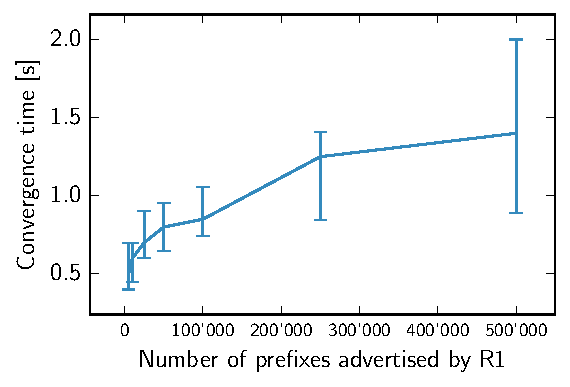
\includegraphics[scale = 1]{Figures/swift.pdf}
\end{minipage}\hfill
\begin{minipage}[t]{.4\textwidth}
\centering
\vspace{0pt}
\begin{tabular}{@{}lr@{}}
	\\
	prefixes & Conv. time \\
	\hline
	\\
    5K & 0.5 s  \\
    10K & 0.6 s   \\
    25K & 0.7 s   \\
    50K & 0.8 s  \\
    100K & 0.85 s \\
    250K & 1.25 s   \\
    500K & 1.4 s  \\
\end{tabular}
\end{minipage}
\caption{Convergence time of the iSDX without Swift}
\label{fig:withswift}
\end{figure}

Figure~\ref{fig:withswift} shows the convergence time in relation to the number of prefixes injected by bgpsimple.
The convergence time increases slightly with higher number of prefixes. At 500'000 prefixes the iSDX takes about 1.5 seconds to push the FR rules. After these 1.5 seconds packets sent from A1 get redirected to C1 and reach their destination. 

\begin{figure}[h]
\center
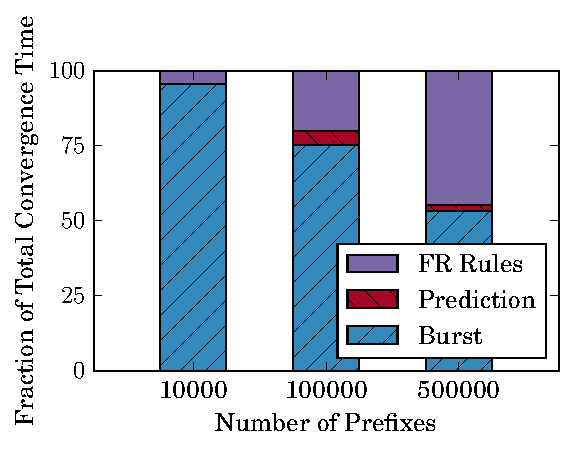
\includegraphics[scale = 1]{Figures/barplot.pdf}
\caption{Time spent on detection, prediction and reroute rule installation during a fast reroute}
\label{fig:activities}
\end{figure}

Figure~\ref{fig:activities} shows what the convergence time is made up of. In blue is the time until a burst of withdrawals is detected. In red is the time it takes to predict the failed AS-link. In violet is the time after the Swift-BPA sends FR messages until the participant controller receives and pushes the FR rules. With a higher number of prefixes withdrawn rises the time until Fast Reroute rules are pushed. The time for the prediction increases slightly with a higher number of prefixes. The time to detect the burst is more or less constant since we used the same Swift configuration for all the experiments. 

\section{\label{chapter5:Swift overhead}Swift Overhead}

In this section we present the overhead that Swift adds to the processing of a single BGP update. We measure the time between the BGP update arriving in the route server and the participant controller finishing to process the update. To measure this we use R1 to advertise a single route and set the link between B1 and R1 down and then up. This gives A1 a single withdrawal and then a single announcement to process. 

\begin{figure}[h]
\center
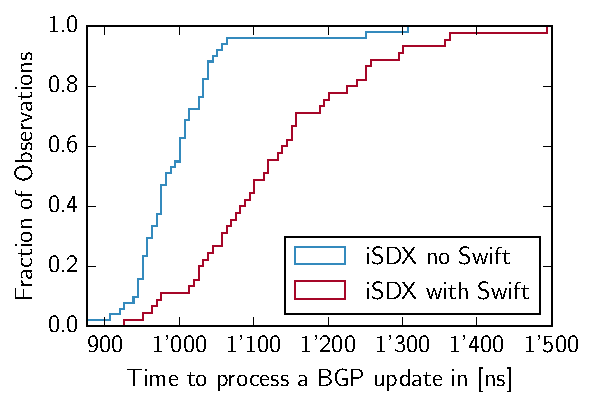
\includegraphics[scale = 1]{Figures/cdf.pdf}
\caption{Time to process a single BGP Update with and without Swift}
\label{fig:swiftoverhead}
\end{figure}

Figure~\ref{fig:swiftoverhead} shows the time to process a single BGP update. On average iSDX takes $987$\,ns without Swift and $1119$\,ns with Swift. We see that Swift increases the processing time by a factor $1.13$.

\newpage